
\chapter{Appendix A: An Example Appendix}%Be sure to include the Heading Appendix A: before you type the name of the Appendix.

\renewcommand{\thechapter}{A} %If you add another appendix, copy and paste this line, but update it to B instead of A.

Appendices should appear at the very end of your thesis. Make sure to label each Appendix with a letter starting with "A". Any tables and/or figures located in the appendix should be labeled accordingly. For example, below is figure A.1 because it is the first figure that appears in Appendix A. 


\begin{figure}[ht]
    \centering
    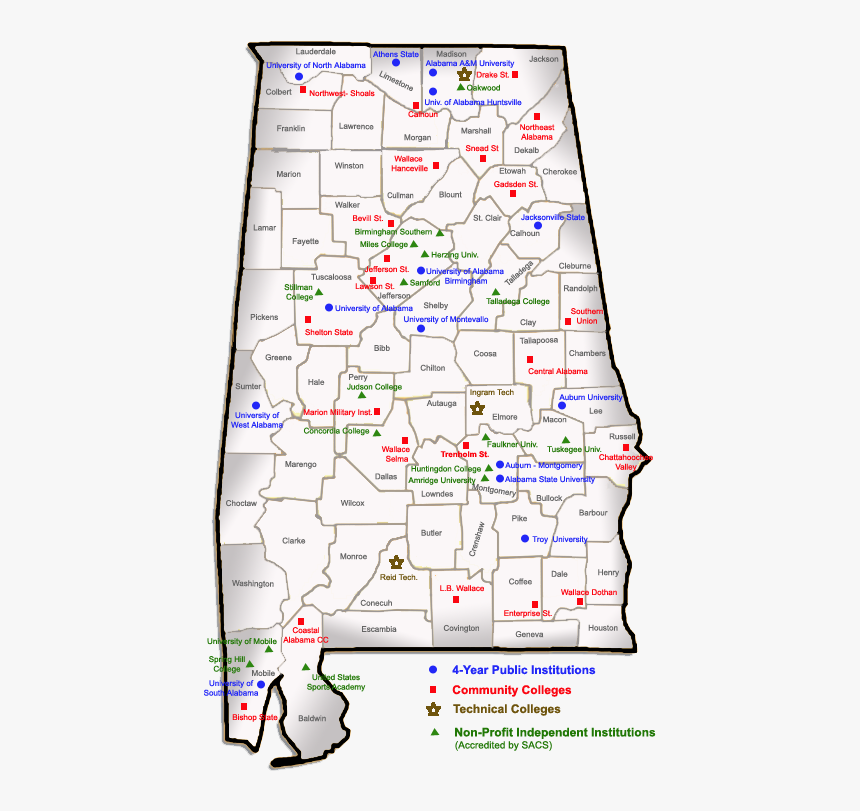
\includegraphics[scale=.4]{Figures/Figure A.1.png}
    \caption[Colleges and Universities in Alabama]{Colleges and Universities in Alabama}
    \label{fig a.1}
\end{figure}


